%=================================================%
% Section:                        	              %
%    Results %
%=================================================%

\begin{center}
\section{Expansion of the Discrete Maximum Principle}
\end{center}

\aboveSubSecSkip
\subsection{Introduction}
\noindent
	\indent 
The findings presented in this work center around four major adjustments to the \gls{dmp}: removing an equilibirum assumption, reducing the complexity of the estimated deposited energy, handling multiple temperature gradients on a single cell's coundaries, and applying multigroup frequency approximations.

One of the assumptions originally made in \cite{WolLarDen} is initial equilibrium between the material and radiation temperatures at the start of each time step.  While this is physically reasonable in most circumstances, we consider the \gls{dmp} more flexible if this assumption is removed.

The term $R$, signifying the estimated energy deposited in a cell over a time step from neighboring cells, exists in previous work as a almost-unmanagably large term involving a combination of operators and integrals.  Because the \gls{dmp} is intended to be used as a predictive warning for existing use codes, it is critical that the prediction does not significantly slow the overall problem simulation.  This makes reducing $R$ to a more manageable, code-friendly set of terms desirable.  We will analyze the components of $R$ and approximate $R$ by removing components that do not significantly effect its value over a wide range of time and spatial steps.

In previous work, the \gls{dmp} was only applied to a one-dimensional Marshak wave problem, where a single source impinged on a single side of the material.  While this has been effective to demonstrate the predicting capacity of the \gls{dmp}, it is conceivable that a simulation involving two hot cells bordering a cold cell may result in a violation of the maximum principle, even when neither hot cell might produce a violation independently.  We will assume linear superposition of energy deposition to derive a multiple-dimension adjustment that improves predictive capacity of the \gls{dmp}.

Lastly, previous computation of the \gls{dmp} has involved using a semi-analytic integration routine.  As part of integrating the \gls{dmp} into use code, we find it prudent to adapt the \gls{dmp} to rely on multigroup frequency approximations similar to those used in the implicit Monte Carlo solver itself.  As we will show, this approximation not only makes the \gls{dmp} easier to implement, but also reduces computation time and increases predictive accuracy.
\belowSubSecSkip

%%%%%%%%%%%%%%%%%%%%%%%%
%
%      Non-Equilibrium
%
%%%%%%%%%%%%%%%%%%%%%%%%
\aboveSubSecSkip
\subsection{Non-Equilibrium Initial Conditions}
\noindent
	\indent 
Parallel to the derivation performed in \cite{WolLarDen}, we consider a single time step, for instance the first step $0\leq t\leq t_1$.  All future time steps $t_n\leq t\leq t_{n+1}$ can be treated in a similar fashion.  Opacity and specific heat are treated explicity at $t=0$ as $\sigma_0$ and $c_{v0}$ respectively.  We retain the definitions from \cite{WolLarDen}:\\
\begin{subequations}\label{defs}
\begin{align}
B(\nu,T) & =\mbox{Planck spectrum}
  =\frac{15ac}{4\pi^5}\frac{\nu^3}{e^{\nu/T}-1},\\
b(\nu,T) & =\mbox{normalized Plank spectrum}
  =\frac{15}{\pi^4T^4} \frac{\nu^3}{e^{\nu/T}-1}, \\
\sigma(\nu,T) & =\mbox{absorption opacity}=\frac{\gamma}{\nu^3}(1-e^{-\nu/T}),\\
\sigma_p &
  =\int_0^\infty b(\nu,T_0)\sigma(\nu,T_0)d\nu=\frac{15\gamma}{\pi^4T_0^3},\\
f_0 & =\mbox{Fleck factor}=\frac{1}{1+\beta_0\sigma_0c\Delta_t},\\
\beta_0 & =\frac{\partial aT_0^4/\partial T}{\partial
  c_{v0}T_0/\partial T}=\frac{4aT_0^3}{c_{v0}},\\
a & =\mbox{radiation constant}=0.01372 \frac{\mbox{jk}}{\mbox{cm$^3$keV$^4$}},\\
c & =\mbox{speed of light}=299.792458 \mbox{cm $/$ sh}.
\end{align}
\end{subequations}
With Eqs. \eqref{defs} defined and moving to a 1-dimensional geometry in the
$x$-direction, Eqs. \eqref{eqn:rtt1} and \eqref{eqn:rtt2} take the following
form, dropping dependency notation:
\begin{subequations}\label{time_start}
\begin{align}
\frac{1}{c}\frac{\partial I}{\partial t} + \mu\frac{\partial I}{\partial x}
+\sigma I =
  \frac{1-f_0}{2}\frac{\sigma_0b_0}{\sigma_p}\int_0^\infty\int_{-1}^1
  \sigma_0 I\ d\mu\ d\nu + &\sigma_0 f_0 2\pi B_0, \nonumber\\& %\hspace{40pt}
  0\leq x\leq\infty,\; |\mu|\leq 1,\; 0\leq t\leq t_1, \label{time_start_1}
\end{align}
\begin{equation}
\frac{c_{v0}}{\Delta_t}(T_1-T_0)=\frac{f_0}{\Delta_t}\int_0^{\Delta_t}
\int_0^\infty\int_ { -1 } ^1
  \sigma_0(I-2\pi B_0)\ d\mu\ d\nu\ dt.
\end{equation}

The initial and boundary conditions are given by:
\begin{equation}
I(0,\mu,\nu,t)=2\pi B_u\equiv2\pi B(\nu,T_u), \hspace{30pt} 
  0<\mu\leq1, \hspace{10pt} 0\leq t, \label{Bu_def}
\end{equation}
\begin{equation}
I(\infty,\mu,\nu,t)=2\pi B_0\equiv2\pi B(\nu,T_0), \hspace{30pt}
  -1\leq\mu\leq1,\hspace{10pt} 0\leq t,
\end{equation}
\begin{equation}
 I(x,\mu,\nu,0)=I_i, \hspace{30pt}0\leq x\leq\infty, |\mu|<1 \label{initcond}.
\end{equation}
\end{subequations}
Eq. \eqref{initcond} is the first deviation from \cite{WolLarDen}, where
the initial intensity was set to the same properties as the right boundary
condition, which assumes complete thermal equilibrium.

We spatially discretize Eqs.\hspace{3pt}\eqref{time_start}
into $J$ distinct
portions, or grid cells, each with a left boundary at $x_j$ and having width
$\Delta_{x,j}=x_{j+1}-x_j$.  The average temperature within each cell is given
by a
temperature averaging function:
\[T_j=\frac{1}{\Delta_{xj}}\int_{x_j}^{x_{j+1}}T(x)dx, \hspace{15pt}
  0\leq j\leq J-1. \]
In this manner, the discontinuous temperature approximation function $\tilde
T(x)$ approximates the physical continuous temperature function $T(x)$ as
follows:
\[\tilde T(x)\equiv\sum_{j=0}^{J-1}\chi_j(x)T_j\approx T(x),\]
where $\chi_j$ is a piecewise distribution, as follows:
\begin{equation}
\chi_j(x)\equiv
\begin{cases}
1 & x_j\leq x\leq x_{j+1}, \\
0 & \mbox{otherwise}.
\end{cases}
\end{equation}
Thus, temperature is often treated in as piecewise constant by
using $\tilde T(x)$ instead of $T(x)$ for explicit terms in Eqs.
\eqref{time_start} such as $\sigma$ and $B$.  The material equation then
appears as follows:
\begin{equation}
\frac{\tilde c_{v0}}{\Delta_t}(T_{j,1}-T_{j,0}) + 
  \tilde f_0 \tilde \sigma_p acT^4_{j,0} = 
  \frac{\tilde f_0}{\Delta_{x,j}
  \Delta_t}\int_0^\infty\tilde\sigma_0\int_{x_j}^{x_{j+1}}
\int_{\Delta_t}\int_{-1}^1 I \ d\mu \ dt\  dx\  d\nu.
\end{equation}

The previous definitions, time-explicit coefficients, and grid data are typical
for the IMC equations.  In the following sections, we introduce additional
approximations in order to estimate the radiation energy deposited in the first
cell.
We start by assuming separability of the radiative
intensity $I$ into the collided ($\breve I$) and uncollided ($\hat I$)
parts so that $\hat I + \breve I=I$.

\subsubsection{Uncollided Intensity}
We approach the uncollided intensity first
because it is more analytically tractable and appears in the collided intensity
equation as a source term. The
following equations govern uncollided intensity:
\begin{subequations} \label{uncollided_1}
\begin{equation}
\frac{1}{c}\frac{\partial\hat I}{\partial t} + \mu\frac{\partial\hat
  I}{\partial x} + \sigma_0\hat I = 0,
\end{equation}
\begin{align}
\hat I(0,\mu,\nu,t)&=2\pi B_u,\hspace{15pt} 0<\mu\leq1, \hspace{10pt}0\leq t,\\
\hat I(\infty,\mu,\nu,t)&=0,\hspace{15pt} -1\leq\mu<0,\hspace{10pt}0\leq t,\\
\hat I(x,\mu.\nu,0)&=0, \hspace{15pt}0\leq x\leq\infty,\hspace{10pt}|\mu|\leq1.
\end{align}
\end{subequations}
Given the lack of any source terms in Eqs. \eqref{uncollided_1}, the
system is completely absorbing in nature.  Iit could be solved
analytically, but will be treated by discretizing in time implicitly:
\[ \frac{1}{c}\left(\frac{\hat I_1-\hat I_0}{\Delta_t}\right) +
  \mu\frac{\partial}{\partial x}\hat I_1 + \sigma_0\hat I_1=0,\]
where $\hat I_k\equiv\hat I(t_k)$ designates the uncollided radiation intensity
at discrete time step $t_k$.  Because of the specified initial condition (i.e.,
all intensity existing at the start of the problem is collided
intensity, the uncollided intensity is zero throughout the mesh at time
$t=0$),
\[\frac{1}{c\Delta_t}{\hat I_1} + \mu\frac{\partial}{\partial x}\hat
I_1 + \sigma_0\hat I_1=0,\]
or, in operator form,
\begin{equation}
\mu\frac{\partial\hat I_1}{\partial x} +
  \left(\sigma_0+\frac{1}{c\Delta_t}\right)\hat I_1 = 0 \label{uncol_ode}.
\end{equation}
For $\mu\geq0$ the solution for the time-implicit uncollided radiation is found
using the integrating factor $e^{\sigma_0x+\frac{1}{c\Delta_t}x}\equiv
e^{\hat\Sigma(\nu)x}$:
\begin{equation}
\hat I_1(x,\mu,\nu)=2\pi B_ue^{-\hat\Sigma x/\mu} \label{uncol_solve}.
\end{equation}
This is limited to particles traveling in angles of positive $\mu$.  This is
practical for a problem with isotropically impinging radiation on once face
of a cell; however, further treatment is necessary in order to
account for significant influences on multiple faces of a cell.  This will be
addressed in Section \ref{propagate} for both single- and multidimensional
cases.

Taking the zeroth angular moment of Eq. \eqref{uncol_solve},
\[\hat\phi_1(x,\nu)\equiv\int_{-1}^1\hat I_1d\mu =
  \int_0^1 2\pi B_ue^{-\hat\Sigma x/\mu}d\mu,\]
\begin{equation} \label{uncol_mom1}
\hat\phi_1(x,\nu)=2\pi B_uE_2(\hat\Sigma x).
\end{equation}
where $E_n$ is the exponential integral defined as follows:
\[E_n(x)\equiv\int_0^1\mu^{n-2}e^{-x/\mu}d\mu,\hspace{15pt}0<x.\]

Eq.\ \eqref{uncol_mom1}, is the approximate solution of the
uncollided intensity.  Note that this derivation coincides precisely with the
process employed by Wollaber, Larsen, and Densmore \cite{WolLarDen}.

\subsubsection{Collided Intensity}
It is in this section that the deviation from previous derivation of the
discrete maximum principle occurs.  Because the collided intensity contains
all the source terms, it is more difficult to treat.  Eqs.
\eqref{collided} are the governing equations of the collided intensity:
\begin{subequations}\label{collided}
\begin{equation}
\frac{1}{c}\frac{\partial\breve I}{\partial t} + 
  \mu\frac{\partial\breve I}{\partial x} + \sigma_0\breve I =
  \frac{1-f_0}{2}\frac{\sigma_0b_0}{\sigma_p}\int_0^\infty\int_{-1}^1
    \sigma_0(\hat I+\breve I)d\mu d\nu +
  2\pi\sigma_0f_0B_0,
\end{equation}
\begin{align}
\breve I(0,\mu,\nu,t)&=0,\hspace{15pt} 0<\mu\leq1, \hspace{10pt}0\leq t,\\
\breve I(\infty,\mu,\nu,t)&=2\pi B_R,\hspace{15pt}
  -1\leq\mu<0,\hspace{10pt}0\leq t,\\
\breve I(x,\mu,\nu,0)&=I_i(x,\mu,\nu), \hspace{15pt}0\leq
  x\leq\infty,\hspace{10pt}|\mu|\leq1 \label{initcond2}.
\end{align}
\end{subequations}
Note that Eq.\ \eqref{initcond2} is the general initial condition employed
particular to this derivation.

To solve Eqs.\ \eqref{collided}, a standard diffusion approximation is
made, leading to the following:
\begin{equation}\label{diff_appr}
\frac{1}{c}\frac{\partial\breve\phi}{\partial t} -
  \frac{1}{3\sigma_0}\frac{\partial^2\breve\phi}{\partial x^2} +
  \sigma_0\breve\phi =
  (1-f_0)\frac{\sigma_0b_0}{\sigma_p}
    \int_0^\infty\sigma_0(\hat\phi+\breve\phi)d\nu +
  4\pi f_0\sigma_0B_0,
\end{equation}
where the scalar intensity $\breve\phi$ is
\[ \breve\phi(x,\nu,t)\equiv\int_{-1}^1\breve I(x,\mu,\nu,t)d\mu.\]
As in \cite{WolLarDen}, it is assumed that $\breve\phi$ has a frequency shape
given
by the Planckian spectrum $b_0$ for cell temperature $T_0$, allowing it to be
separated as follows:
\[\breve\phi(x,\nu,t)\approx b_0(\nu)\check\phi(x,t).\]
Defining the diffusion coefficient
\begin{equation}
D\equiv\int_0^\infty\frac{b_0(\nu)}{3\sigma_0(\nu)}d\nu,\label{defD}
\end{equation}
Eq. \eqref{diff_appr} can be integrated over all frequencies $\nu$ to
obtain
\begin{equation} \label{diff2}
\frac{1}{c}\frac{\partial\check\phi}{\partial t}
  -D\frac{\partial^2\check\phi}{\partial x^2} + f_0\sigma_p\check\phi
  =(1-f_0)\int_0^\infty\sigma_0\hat\phi d\nu + f_0\sigma_pacT^4_0.
\end{equation}
At this point, an implicit time discretization is
employed, although the approach is more general here given the undefined
initial condition throughout the mesh given in Eqs.\ \eqref{collided}. 
Implicit time discretization is employed as follows for any time-dependent
function $f(t)$:
\[ \bar f(t) \equiv\frac{1}{\Delta_t}\int_{t_n}^{t_{n+1}}f(t) dt 
  \approx f(t_{n+1}).\]
Additionally, we define the radiation temperature at time $t=0$ to satisfy:
\[ \int_0^\infty\check\phi_0\ d\nu\equiv\int_0^\infty\int_{-1}^1\check I_i\
d\mu\ d\nu \equiv acT_R^4,\]
where we define $T_R$ as the radiation field temperature within the cell at
time $t=0$.
Applying time differencing to Eq. \eqref{diff2}, we arrive at the
following:
\begin{equation}
\frac{\partial^2 \check\phi_1}{\partial x^2} - \lambda^2\check\phi_1 =
  \frac{1-f_0}{-D}\int_0^\infty \sigma_0\hat\phi d\nu -
  \frac{acT_R^4}{c\Delta_tD} - \frac{f_0\sigma_p}{D}acT_0^4,
\end{equation}
where $\lambda$ has been
introduced as
\[ \lambda^2\equiv\frac{f_0\sigma_p+1/c\Delta_t}{D}.\]

Using Eq. \eqref{uncol_mom1} in Eq. \eqref{diff2},
\begin{subequations}\label{ode}
\begin{equation}
\frac{\partial^2 \check\phi_1}{\partial x^2} - \lambda^2\check\phi_1 =
  \frac{1-f_0}{-D}\int_0^\infty\sigma_02\pi B_uE_2(\hat\Sigma x) d\nu -
  \frac{acT_R^4}{c\Delta_tD} - \frac{f_0\sigma_p}{D}acT_0^4. \label{ode_main}
\end{equation}
As with \cite{WolLarDen}, a Marshak boundary condition is set at the left:
\begin{equation}
\check\phi_1(0)-2D\frac{d\check\phi_1}{dx}\bigg|_{x=0}=0, \label{marshakBC}
\end{equation}
and the right boundary is
\begin{equation}
\lim_{x\to\infty}\check\phi_1(x)=acT_R^4. \label{infBC}
\end{equation}
To bring this derivation back in harmony with \cite{WolLarDen}, $\tilde A$ is
defined
\begin{equation}
\tilde A\equiv - \frac{acT_R^4}{c\Delta_tD} - \frac{f_0\sigma_p}{D}acT_0^4,
\end{equation}
and operator $L$
\begin{equation}
L(\xi)\equiv\frac{1-f_0}{-D}\int_0^\infty\sigma_02\pi B_u\xi d\nu,\label{defL}
\end{equation}
making Eq.\ \eqref{ode_simple}, the simplification of Eq.\ \eqref{ode_main},
identical in
appearance to Eq. (17g) in \cite{WolLarDen}:
\begin{equation}\label{ode_simple}
\frac{\partial^2\check\phi_1}{\partial x^2}-\lambda^2\check\phi_1 =
  \tilde A + L\left(E_2(\hat\Sigma x)\right).
\end{equation}
\end{subequations}
\\
We see by inspection that the remainder of the derivation in \cite{WolLarDen}
applies perfectly to
\eqref{ode_simple}, only trivially replacing $A$ everywhere with $\tilde A$. 
The final results arrived at in \cite{WolLarDen} are shown here, noting only
that $\tilde R$ (the average energy deposited in the first cell) and $\tilde A$
contain the radiation temperature $T_R$ as well as the material temperature
$T_0$.
\begin{align}\label{R}
\tilde R(\Delta_x,\Delta_t)&\equiv\frac{f_0\Delta_t2\pi}{\Delta_x}
  \int_0^\infty\frac{\sigma_0B_u}{\hat\Sigma}\left(\frac{1}{2}-
    E_3(\hat\Sigma\Delta_x)\right)d\nu \nonumber\\
  &+\frac{c_1f_0\Delta_t\sigma_p}{\lambda\Delta_x}(1-e^{-\lambda\Delta_x}) +
  \frac{f_0\Delta_t\sigma_p}{\lambda^2\Delta_x}\left[-\tilde A\Delta_x
    -L\left\{\frac{1}{\hat\Sigma}\left(\frac{1}{2}
    -E_3(\hat\Sigma\Delta_x)\right)\right\}\right] \\
  &\hspace{15pt}+\frac{f_0\Delta_t\sigma_p}{\Delta_x\lambda^4}L\Bigg\{\hat\Sigma
    \bigg[e^{-\lambda\Delta_x}\mbox{Ei}[(\lambda-\hat\Sigma)\Delta_x] +
    e^{\lambda\Delta_x}\mbox{Ei}[-(\lambda+\hat\Sigma)\Delta_x] \nonumber \\
  &\hspace{140pt} -2\mbox{Ei}(-\hat\Sigma\Delta_x)+ \nonumber
    \ln\frac{\hat\Sigma^2}{(\lambda+\hat\Sigma)|\lambda-\hat\Sigma|}
    \bigg]\Bigg\},
\end{align}
Thus, the IMC equations can be expected to satisfy the maximum principle if the
following inequality is satisfied, calculating $\tilde R$ as in Eq.\ \eqref{R}.
\begin{equation}\label{DMP}
\Delta_t<\frac{c_v(T_u-T_0)}{\tilde
R(\Delta_x,\Delta_t)-f_0c\sigma_paT_0^4}.
\end{equation}
Eq.\ \eqref{DMP} represents the \gls{dmp} without assuming initial equilibrium between the radiation and material temperatures.



%%%%%%%%%%%%%%%%%%%%%%
%
%        Reducing R
%
%%%%%%%%%%%%%%%%%%%%%%


\aboveSubSecSkip
\subsection{Analysis of $R$}
Continuing from Eq.\ \eqref{DMP}, we seek a functional form more agreeable for use in a coding environment. 
Primarily, this involves approximating computationally difficult functions such as the
exponential integrals $E_n(x)$ and $\mbox{Ei}(x)$, as well as numerically
evaluating
the various integrals over frequency.

\subsubsection{Approximating $\tilde R$}
We address each of the terms of $\tilde R$ by breaking them up in Eq.
\eqref{DMPsplit}:
\begin{subequations}\label{DMPsplit}
\begin{align}
\tilde R(\Delta_x,\Delta_t)&\equiv\frac{f_0\Delta_t2\pi}{\Delta_x}
  \int_0^\infty\frac{\sigma_0B_u}{\hat\Sigma}\left(\frac{1}{2}-
    E_3(\hat\Sigma\Delta_x)\right)d\nu \label{DMP1}\\
  &+\frac{c_1f_0\Delta_t\sigma_p}{\lambda\Delta_x}(1-e^{-\lambda\Delta_x})
    \label{DMP2}\\
  &+\frac{f_0\Delta_t\sigma_p}{\lambda^2\Delta_x}\left[-\tilde A\Delta_x
    -L\frac{1}{\hat\Sigma}\left(\frac{1}{2}
    -E_3(\hat\Sigma\Delta_x)\right)\right] \label{DMP3}\\
  &\hspace{15pt}+\frac{f_0\Delta_t\sigma_pL}{\Delta_x\lambda^4}\hat\Sigma
    \bigg[e^{-\lambda\Delta_x}\mbox{Ei}[(\lambda-\hat\Sigma)\Delta_x] +
    e^{\lambda\Delta_x}\mbox{Ei}[-(\lambda+\hat\Sigma)\Delta_x] \label{DMP4} \\
  &\hspace{140pt} -2\mbox{Ei}(-\hat\Sigma\Delta_x)+ \nonumber
    \ln\frac{\hat\Sigma^2}{(\lambda+\hat\Sigma)|\lambda-\hat\Sigma|} \bigg].
\end{align}
\end{subequations}
While the terms in Eq. \eqref{DMPsplit} are generally listed in order of
increasing powers of $\lambda$ in the denominator, it should be noted that term
\eqref{DMP2} actually contains the term $\lambda^4$, because of the definition
of $c_1$ in Eq. (31) of \cite{WolLarDen}:
\[c_1=\frac{1}{1+2D\lambda}\frac{1}{\lambda^2}\left[A + 
  L\left(1+\frac{\hat\Sigma}{2\lambda}\ln\frac{|\lambda-\hat\Sigma|}{\lambda +
  \hat\Sigma} \right) \right],\hspace{10pt}\lambda\neq\hat\Sigma. \]

Inspection of the definition of $\lambda$ (repeated below) assists in assigning
the relative importance of terms in Eq. \eqref{DMPsplit}:
\[\lambda^2\equiv\frac{f_0\sigma_p + 1/c\Delta_t}{D}
  = \frac{f_0\sigma_p}{D} + \frac{1}{Dc\Delta_t} \]
  Since $f_0$ is restricted from zero to one, primary attention is turned to the
other terms in $\lambda^2$.


\subsubsection{Temperature}
Figure \ref{lambdaT} shows
$\lambda^2$ versus temperature for constants $\gamma=27$ keV$^3$/cm,
$c=3\times10^2$
cm/sh, and $\Delta_t=10^{-5}$ sh.  Additionally, it is assumed that the Planck
opacity
has the functional form
\begin{equation}
\sigma_p=\frac{15\gamma}{\pi^4T_0^3}\label{sigp assum},
\end{equation}
which may not be valid for many real materials, but serves as a
physically viable test case.

\begin{figure}[htb]
\centering
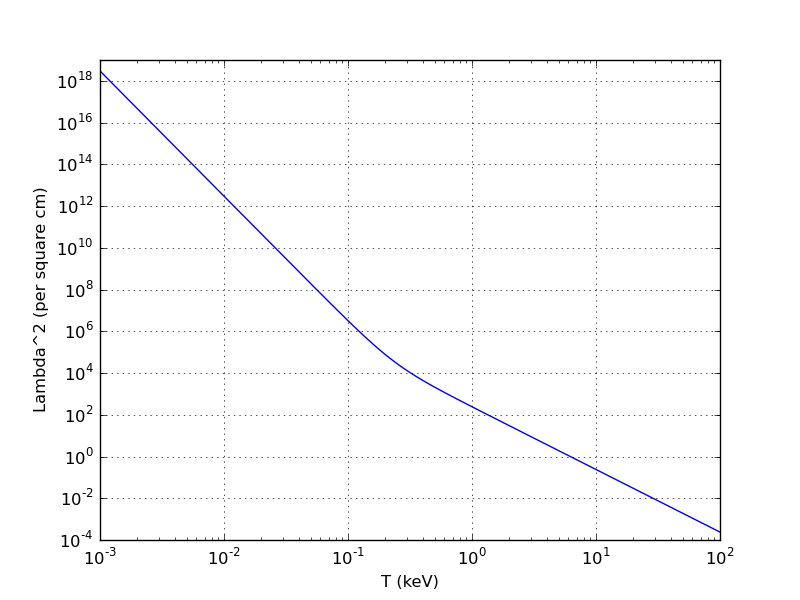
\includegraphics[width=0.7\linewidth]{graphics/lambdaT}
\caption{$\lambda$ as a function of material temperature}
\label{lambdaT}
\end{figure}
As can be seen, $\lambda^2$ falls as $T^6$ until an inflection point is reached
near $T=0.3$ keV, after which it falls as $T^3$.  It is worth noting that for
most of the range $0<T<1$ keV, $\lambda^2$ is very large.  As such, terms in
$\tilde R$ with exponential values of $\lambda^2$ will be vanishingly small for
most temperatures below 1 keV; however, further analysis needs to be done in
order to determine how many terms in $\tilde R$ can be neglected because of
their insignificance next to other terms because of temperature.


\subsubsection{Time Step}
It is also enlightening to consider the effect of an increasing time step on
$\lambda^2$.  Since a 1/$\Delta_t$ term is in the numerator of $\lambda^2$, a
term with 1/$\lambda^2$ varies as $O(\Delta_t)$ as $\Delta_t \to \infty$.  In
Eq.\
\eqref{DMPsplit}, a $\Delta_t$ term already exists in the numerator of each
term.
Thus, term\ \eqref{DMP1} varies linearly with $\Delta_t$.  The term with the
next lowest order of $\lambda$, term\ \eqref{DMP3}, has a 1/$\lambda^2$
coefficient, meaning it varies as $\Delta_t^2$.  Terms\ \eqref{DMP2} and\
\eqref{DMP4} vary as $\Delta_t^{5/2}$ and $\Delta_t^3$ respectively.  Thus, as
the time step becomes large, the latter terms in Eq.\ \eqref{DMPsplit} become
more significant.

It is unclear from the influence of both $T$ and $\Delta_t$ what terms in
$\tilde R$ are necessary to maintain accuracy for a variety of conditions. 
Future work will be done to evaluate these terms independently in the limit as
$\Delta_t\to 0, \infty$.  For the sake of the current work,
we turn to numerical methods to evaluate the relative impact of the terms,
acknowledging the results are specific to this particular sample problem.

\subsubsection{Numerical Comparison}
Given the difficulty in analytically determining the importance of the terms in
$\tilde R$, we performed a numerical study similar to that in \cite{WolLarDen},
using the
same values for $\sigma_p$, $\beta$, and $D$.  In each run, one of the terms
in
Eq.\ \eqref{DMPsplit} was set to zero, with the exception of the first term,
which si the dominant contributor to $\tilde R$ for this problem.  Instead, the
first term
was reduced by an order of magnitude in order to show how it scales the overall
calculation of the
discrete maximum principle.  The results are shown in Figures \ref{numR} through
\ref{numR_relErr} with the following definition for each case:
\begin{center}
\begin{tabular}{c c l}
Run & Modified Term & Modification  \\ \hline \medskip
All Terms & None &  None\\ \medskip
Case 0    & $\int_0^\infty2\pi B_u\frac{\sigma_0}{\hat\Sigma}
  \left(\frac{1}{2}-E_3(\hat\Sigma\Delta_x)\right)\ d\nu $& $\to 0$ \\ \medskip
Case 1    & $\frac{\sigma_p}{\lambda^2}L\frac{1}{\hat\Sigma}
  \left(\frac{1}{2}-E_3(\hat\Sigma\Delta_x)\right)\;$& \textdiv 10  \\ \medskip
Case 2    & $\frac{c_1\sigma_p}{\lambda\Delta_x} 
  \left(1-e^{-\lambda\Delta_x}\right) $ &$\to0$ \\ \medskip
Case 3    & $\frac{\sigma_p}{\lambda^2}A\Delta_x $ &$\to0$  \\ \medskip
Case 4    & Term\ \eqref{DMP4} & $\to0$  \\ \medskip
Case 5    & Cases 2, 3, and 4 combined &$\to0$
\end{tabular}
\end{center}
As can be seen, Case 1 had the greatest impact, followed by
Case 0, with Case 3 in a distant third place.  The terms
eliminated in Cases 2 and 4, on the other hand, seem to have very little real
impact on the overall location of the maximum principle violations.  In order to
minimize computation,
the terms left out in cases 2 and 4 will be left out of the
implementation of the DMP.

\begin{figure}[H]
\centering
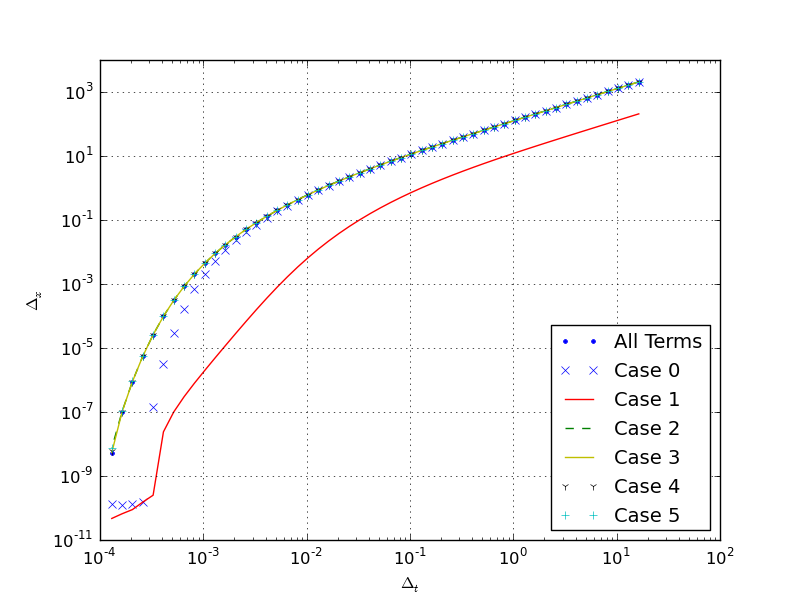
\includegraphics[width=0.7\linewidth]{graphics/numR}
\caption{Energy Deposited, $R$}
\label{numR}
\end{figure}

\begin{figure}[H]
\centering
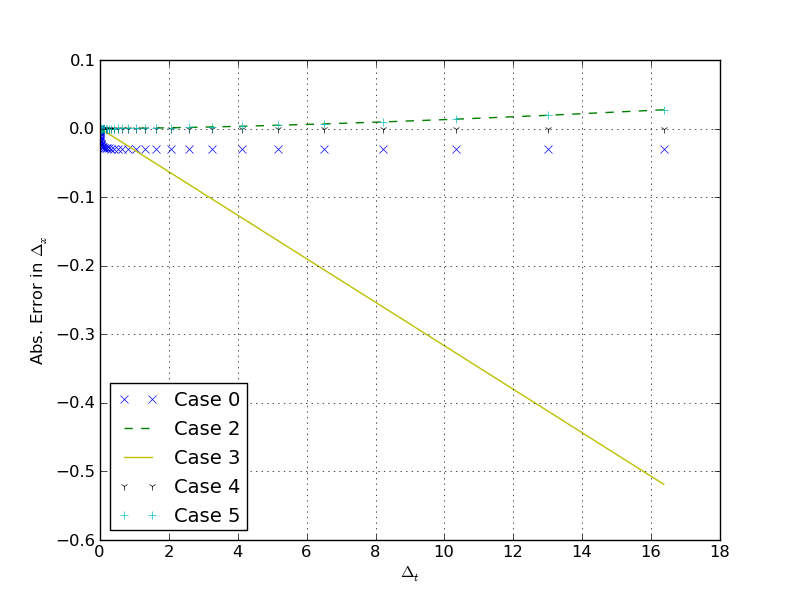
\includegraphics[width=0.7\linewidth]{graphics/numR_absErr}
\caption{Absolute Error in $R$ Approximations}
\label{numR_absErr}
\end{figure}

\begin{figure}[H]
\centering
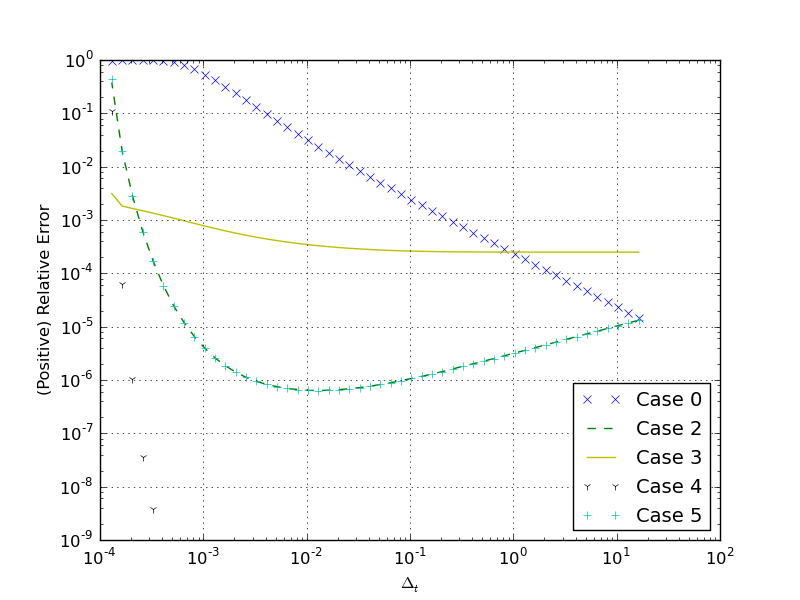
\includegraphics[width=0.7\linewidth]{graphics/numR_relErr}
\caption{Relative Error in $R$ Approximations}
\label{numR_relErr}
\end{figure}
\noindent
Removing the two least-significant terms in $R$, we can rearrange to get
\begin{equation}
\tilde R\simeq\frac{f_0\Delta_t}{\Delta_x}\left(\zeta -
  \frac{\sigma_p}{\lambda^2}\tilde A\Delta_x - 
  \frac{\sigma_p}{\lambda^2}\frac{1-f_0}{-D}\zeta\right), \label{R approx}
\end{equation}
where we define the uncollided flux integral
\begin{equation}
\zeta\equiv\int_0^\infty 2\pi\sigma_0B_u\left[
  \frac{1}{2}-E_3(\hat\Sigma\Delta_x)\right]\ d\nu. \label{UncollidedFlux}
\end{equation}

\belowSubSecSkip


%%%%%%%%%%%%%%%%%%%%%%
%
%      Multiple Gradients
%
%%%%%%%%%%%%%%%%%%%%%%
\aboveSubSecSkip
\subsection{Multiple Gradients}
Thus far we have assumed a one-dimensional problem with a Marshak boundary on the
left and a generally uninteresting right boundary condition. 
This allowed us to assume only steep temperature gradients on one side of the
left boundary cell during the first time step. We now desire to apply the DMP in
general to each cell in the mesh, so
that an inequality similar to Eq.\ \eqref{DMP} can be computed for a cell with
steep temperature gradients on
multiple sides.  We will do this by accounting for impingent radiation on
multiple faces of a cell in our approximation of $\tilde R$, although we will continue to treat the radiation as
being isotropic and Planckian.  The primary result of the Marhsak boundary assumption
allowed us to
find the solution in Eq.\ \eqref{uncol_solve}.  This was then used to calculate
the uncollided scalar intensity $\hat\phi_0$.  In the 1D case, $\hat\phi_0$ can
be restated as follows:
\begin{equation}
\hat\phi_1\equiv\int_{-1}^1 \hat I_i\ d\mu = \int_{-1}^0 \hat I_i\ d\mu + 
  \int_0^1 \hat I_i\ d\mu. \label{uncol_gen}
\end{equation}
Because the initial conditions prescribe no uncollided intensity in a cell
initially, the intensity present at a point $x$ can only originate from incident
intensity on the boundaries.  The differential equation describing this is
given in Eq.\ \eqref{uncol_ode} and is solved in Eq.\ \eqref{uncol_solve}. 
There is physical meaning to the terms: $2\pi B_u$ represents the initial
spectrum of intensity found at the Marshak boundary entering the cell, and
$e^{-\Sigma x/\mu}$ attenuates this intensity through material interactions up
to point $x$.  Hence, a similar expression for uncollided flux arriving at $x$
from the right boundary can be derived as well.

Let $B_L$ replace $B_u$ as the Planck radiation spectrum on the left boundary,
and let $B_R$ represent a similar spectrum on the right boundary.  Similarly
let $\hat I_{L,i}$ and $\hat I_{R,i}$ represent the incident uncollided
intensity at the left and right right boundary, respectively.  Eq.\
\eqref{uncol_mom1} becomes
\begin{align}
\hat\phi_1&\equiv\int_{-1}^1 \hat I_i\ d\mu \nonumber ,\\
&=\int_{-1}^0 \hat I_{R,i}\ d\mu + 
  \int_0^1 \hat I_{L,i}\ d\mu \nonumber ,\\
&=\int_{-1}^0 \hat I_{R,i}\ d\mu +
  \int_0^1 2\pi B_Le^{-\hat\Sigma x/\mu}\ d\mu. \label{uncol_gen2}
\end{align}
Because of the arbitrary definition of positive $\mu$, we expect $\hat I_{R,i}$
to have a similar form to $\hat I_{L,i}$.  However, the attenuation term must
be treated differently for negative $\mu$ radiation.  Because the radiation
enters at the right and moves to the left, the attenuation distance for the
right side becomes $\Delta_x-x$. Thus by inspection and symmetry,
\begin{equation}
\int_{-1}^0 \hat I_{R,i}\ d\mu
  =\int_{-1}^0 2\pi B_R e^{-\hat\Sigma(\Delta_x-x)/\mu}\ d\mu.\label{IR1}
\end{equation}
To continue shaping this new first term to correlate with the second term,
consider that in the first integral all values of $\mu$ are negative.  Given
this condition,
\[\mu=-|\mu|, \hspace{30pt} \mu\leq0.\]
Substituting this into Eq.\ \eqref{IR1} and making a change of integration
variable to $|\mu|$, we obtain an expression very similar to the second term in
Eq.\ \eqref{uncol_gen2}:
\begin{equation}
\int_{-1}^0 \hat I_{R,i}\ d\mu = \int_0^1 2\pi B_R
  e^{-\hat\Sigma(x-\Delta_x)/|\mu|}\ d|\mu|.
\end{equation}
Since the new attenuation coefficient is identical in form to that in Eq.\
\eqref{uncol_solve}, the integral solution has the same form.  Thus,
\begin{equation}
\hat\phi_1=2\pi B_LE_2(\hat\Sigma x) +
  2\pi B_RE_2\left(\hat\Sigma(\Delta_x-x)\right) \label{phi1_LR}
\end{equation}
Eq.\ \eqref{phi1_LR} is sufficiently different from Eq.\ \eqref{uncol_solve}
that the original operator $L$ is divided into an operator $L_L$ for the left
side and $L_R$ for the right:
\begin{subequations}
\begin{align}\label{L_LR}
L_L(\xi)&\equiv\frac{1-f_0}{-D}\int_0^\infty\sigma_02\pi B_L\xi\ d\nu, \\
L_R(\xi)&\equiv\frac{1-f_0}{-D}\int_0^\infty\sigma_02\pi B_R\xi\ d\nu,
\end{align}
\end{subequations}
which, using the same procedure as in \cite{WolLarDen}, leads to a new
particular solution for $\breve\phi_1$:
\begin{align}
\breve\phi^p_1=\frac{1}{\lambda^2}\bigg[
  &-A-L_RE_2(\hat\Sigma(x-\Delta_x))+L_R\frac{\hat\Sigma}{2\lambda}\left(
    e^{-\lambda x}g(x-\Delta_x)+
    e^{\lambda x}E_1[(\lambda+\hat\Sigma)(\hat\Sigma(x-\Delta_x))]
    \right)\nonumber\\
  &-L_LE_2(\hat\Sigma x)+L_L\frac{\hat\Sigma}{2\lambda}\left(
    e^{-\lambda x}g(x)+e^{\lambda x}E_1[(\lambda+\hat\Sigma)x]\right)\bigg],
\end{align}
where
\begin{equation}
g(x)\equiv\int\frac{e^{(\lambda-\hat\Sigma)x}}{x}dx=
\begin{cases}
\mbox{Ei}[(\lambda-\hat\Sigma)x], & \lambda\neq\hat\Sigma, \\
\ln{x}, & \lambda=\hat\Sigma,
\end{cases}
\end{equation}
which makes use of the extension to Ei(x) noted in \cite{MathFunc}:
\[\mbox{Ei}(-x)\equiv-E_1(x),\; 0<x.\]

Next we apply the Marshak and finite boundary conditions.  The homogeneous
solution for $\breve\phi_1$ is the same as derived earlier, and we still set
$c_2=0$ to preserve the condition in Eq.\ \eqref{infBC}.  After some algebraic
manipulation, and noting the convenient equal divergence and limits described
in \cite{WolLarDen}, it can be shown that the average energy deposited in a
cell ($\tilde R$) follows the superposition principle for left and right sides
of the cell.  That is to say,
\[\tilde R = \tilde R_L + \tilde R_R.\]

The temperature update in a cell then becomes
\[\frac{c_v}{\Delta_t}(T_1-T_0)+f_0c\sigma_p aT_0^4=\tilde R_L+\tilde R_R,\]
\begin{equation}
T_1-T_0=\frac{\Delta_t}{c_v}(\tilde R_L+\tilde R_R-f_0c\sigma_p aT_0^4).
\label{tempUpd}
\end{equation}
Two separate equations fall out of Eq.\ \eqref{tempUpd}, one for each side of
the cell.  Since both the left boundary temperature $T_L$ and the right
boundary temperature $T_R$ limit the time step in similar ways, we here
define the maximum temperature
\[T_m\equiv\mbox{max}(T_L,T_R). \]
\begin{equation}\label{boundTempUpd}
T_m-T_1=T_m-T_0-\frac{\Delta_t}{c_v}(\tilde R_L+\tilde R_R-f_0c\sigma_p aT_0^4),
\end{equation}
As in \cite{WolLarDen}, the maximum principle is only satisfied if the boundary
temperature is greater than the update temperature, meaning the right side of
Eq.\ \eqref{boundTempUpd} is positive:
\begin{equation}\label{DMP_LR}
T_m-T_0>\frac{\Delta_t}{c_v}(\tilde R_L+\tilde R_R-f_0c\sigma_p aT_0^4),
\end{equation}
or, rearranging, the maximum principle can be stated in the same form as that
in \cite{WolLarDen},
\begin{equation}
\Delta_t < \frac{c_v(T_m-T_0)}{\tilde R_L(\Delta_x,\Delta_t)+\tilde
  R_R(\Delta_x,\Delta_t) - f_0c\sigma_p aT_0^4},
\end{equation}

It should be noted that the term $T_m-T_0$ in the numerator here is misleading. 
An analysis of the frequency-independent DMP leads to an inequality with
$T_m^4-T_0^4$ in the denominator, for example.

\subsection{Multidimensional Considerations}
Given the results achieved in the one-dimensional case, the maximum principle in
multiple dimensions can be extrapolated by adjusting
$\tilde R$.  Since the average energy deposited ($\tilde R$) is
separable in that it follows superposition rules, the composite term is as
follows:
\begin{equation}
\tilde R_{tot} = \sum_{s=1}^S \tilde R_s(\Delta_x,\Delta_t),
\end{equation}
where $S$ is the number of faces on the cell in question and $s$ represents one
of those faces.

The question of what to use for $\Delta_x$, the spatial discretization, in
higher dimensions is a valid one, and needs addressing.  In one dimension, it is
obvious that the cell size is equal to its length. However, in multiple
dimensions, the cell size is an area or volume, and linear distance
becomes more difficult to define uniquely.  To resolve this, we turn to the work
done by Bardsley and Dubi \cite{BardDub}, who expound the average-chord-length
theorem developed by Dirac \cite{Dirac}. This theorem states that for any
three-dimensional volume, the average chord length within that volume is given
by
\begin{equation}
\bar\Delta_x = 4\frac{V}{A},
\end{equation}
where $V$ is the volume and $A$ is the surface area of the volume.  We use this
definition to describe the value $\Delta_x$ in three dimensions to redefine the
discrete maximum inequality
\begin{equation}
\Delta_t<\frac{c_v(T_m-T_0)}{\tilde R_{tot}(\Delta_x,\Delta_t)-
  f_0c\sigma_paT_0^4},  \hspace{20pt} T_m=\mbox{max}(T_s).\label{FINAL dmp}
\end{equation}
\belowSubSecSkip



%%%%%%%%%%%%%%%%%
%
% Multigroup
%
%%%%%%%%%%%%%%%%%
\aboveSubSecSkip
\subsection{Multigroup Frequencies}
 A ``multigroup approximation'' is often
performed to allow the emission and absorption characteristics of individual energy spectra
to be represented as a sum instead of a continuous integral.  We derive such a
technique here.  Without making
any approximation, the integrated value of a general function $f(\nu)$ can be
represented as
\[\int_0^\infty f(\nu)\ d\nu = \sum_{\nu=0}^\infty f(\nu).\]

We can further split this continuous sum into groups of continuous sums,
still without making any approximations:
\[\int_0^\infty f(\nu)\ d\nu = \sum_{g=0}^\infty f_g,\]
where the group function is defined
\[f_g\equiv\int_g^{g-1} f(\nu)\ d\nu.\]
Note here that lower values of $g$ correspond to higher values of $\nu$.  as is the 
typical convention in multigroup theory.

Since finding the integrated value of $f(\nu)$ is still no easier than before,
we now make an approximation by truncating the infinite sum:
\[\int_0^\infty f(\nu)\ d\nu \approx \sum_{g=0}^G f_g.\]
In the limit that $G\to\infty$, there is no approximation made.

As necessary, further approximation can be made if $f(\nu)$ is separable into
several functions of $\nu$.  For example, let
\[f(\nu) = \frac{A(\nu)B(\nu)}{C(\nu)}.\]
In the multigroup approximation, then,
\[\int_0^\infty f(\nu) \approx \sum_{g=0}^G f_g
   = \sum_{g=0}^G \frac{A_gB_g}{C_g}.\]
This is an approximation in that, for the general case,
\[\int \frac{A(x)B(x)}{C(x)}\ dx
   \neq \frac{\int A(x)\ dx\ \int B(x)\ dx}{\int C(x)\ dx}.\]
However, using these multigroup approximations, previously-inhibiting
integrations can be discretized into terms that can be computed.

\subsubsection{Riemann Approximation}
In this work, a Riemann approximation is used to find the group values for
continuous integrals as described above.  The basic tenet of this approximation
is that continuous integrals may be approximated as the sum of many trapezoidal
figures that roughly approximate the shape of the integrand (see Figure\
\ref{RiemannFig}).  There are several different methods of implementing the
Riemann sum.  The value of the function over a range can be the function
evaluated at the leftmost part of the range, the value at the rightmost part
of the range, or the value in the center of the range.  The approximation in
Figure\ \ref{RiemannFig} is representative of a fourth, more
accurate method: the ``trapezoidal'' method.  In this method, the Riemann
segment an upper value that is the linear-fit average of the function in the
cell instead of the function evaluated at any one point. For this method, the
integral of the function is approximated as
\[\int_a^b f(x)\ dx \approx \sum_{r=1}^R \frac{\big[f(x_r)+f(x_{r+1})\big]
  \Delta r}{2}\]
where $x_r$ is the value of $x$ at the leftmost bound of the Riemann segment.
\begin{figure}[htb]
\centering
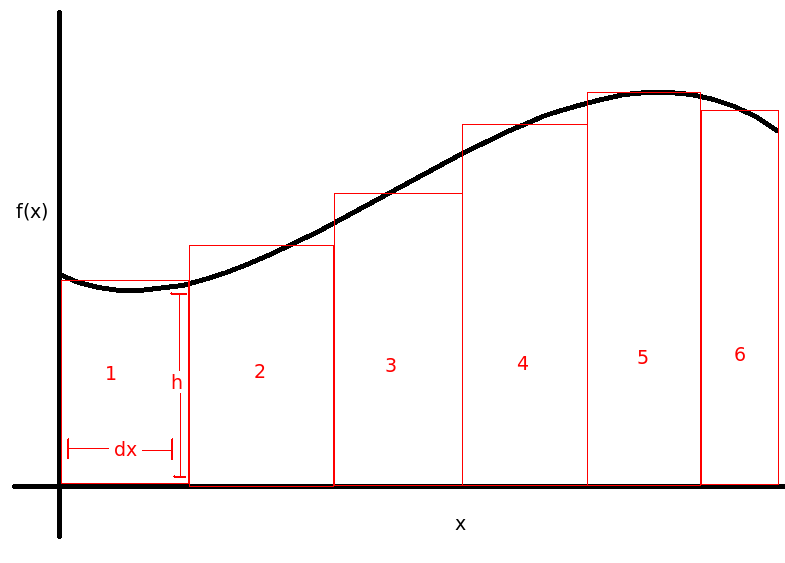
\includegraphics[width=0.7\linewidth]{graphics/RiemannFig}
\caption{Visualization of Riemann Sum Method}
\label{RiemannFig}
\end{figure}

\newpage
\subsubsection{Accuracy of Multigroup Approximation}
In order to compare the multigroup approximation to a more analytic solution,
the DMP was calculated using the multigroup method described above, then with
an analytic solve using the \texttt{MatLab} computer algebra
software. The results are shown in Figure
\ref{mg_vs_anl}. Calculating the relative error between the two methods led to a
machine-precision difference in all cases.  For the large set of runs used to
create the discrete maximum curve shown in Figure \ref{mg_vs_anl}, the analytic
method took about 160 seconds, while the multigroup method took just over 23
seconds, suggesting the multigroup method is on the order of seven times faster
to calculate than the analytic method.
\begin{figure}[htb]
\centering
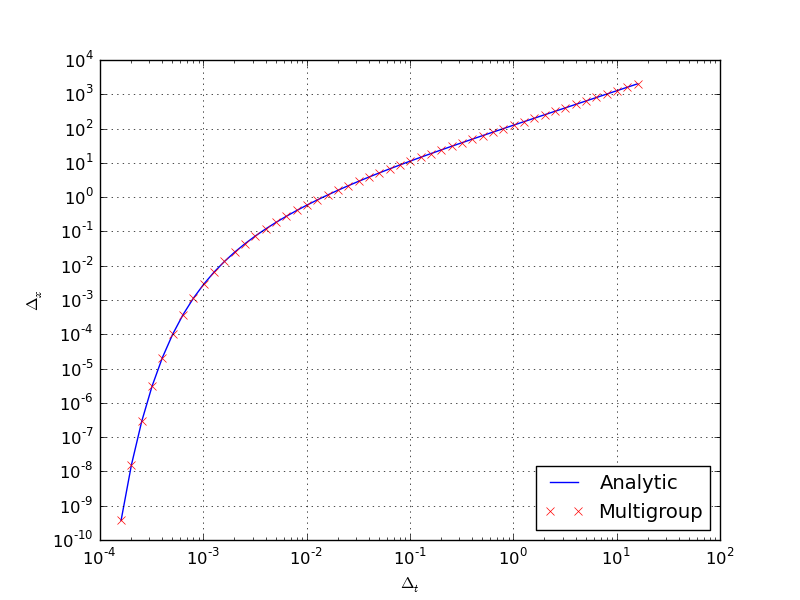
\includegraphics[width=0.7\linewidth]{graphics/DMP_mg_numR}
\caption{Multigroup versus Analytic Solutions for the DMP}
\label{mg_vs_anl}
\end{figure}

Using this  multigroup approximation technique
and the numerical solution for $E_3(\hat\Sigma\Delta_x)$ discussed in
Appendix \ref{apxEn}, Eq.\ \eqref{R approx} becomes computationally
straightforward.

An interesting result occurs when the multigroup approximation is applied to
the estimate $\tilde R$.  In Figure \ref{CMP_DMP} we note that the analytic
Discrete Maximum
Principle curve, obtained from a numerical integral over frequency in
\texttt{Matlab}, diverges from the experimental data somewhere between
$\Delta_t$ of 0.001 and 0.01 shakes.  This suggests that the analytic discrete
maximum principle is not conservative enough to match experiment.  However,
when the multigroup approximation is applied, the curve matches much more
closely, as shown in Figure \ref{mg_DMP}.  It is not entirely surprising that
the multigroup approximation is more accurate, since
the experimental results were generated using a 100-group frequency grid in
\gls{imc} use code \texttt{milagro}.
\begin{figure}[htb]
\centering
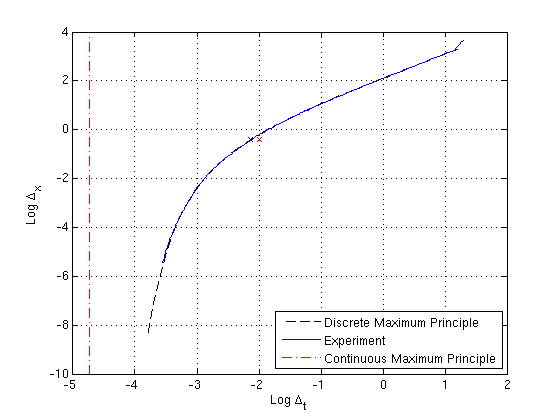
\includegraphics[width=0.7\linewidth]{graphics/grossMG}
\caption{Multigroup Approximation of DMP}
\label{mg_DMP}
\end{figure}


\subsubsection{Grey Case}
Because of the structure of the use codes that the DMP will likely be used in,
we deem it essential to construct an algorithm that will handle the 1-group gray
case as well as the multifrequency case.  A derivation of the discrete maximum 
principle for the frequency-independent gray case is derived here that takes
the same form as Eq.\ \eqref{DMP}.

We start with the gray transport equation in one dimension in \cite{FleckCumm},
which assumes that frequency is independent of angle and can be integrated out:
\begin{equation}
\frac{1}{c}\frac{\partial I}{\partial t} + \mu\frac{\partial I}{\partial x} +
  \sigma_0 I = \sigma_0(1-f_0)\frac{1}{2}\int_{-1}^1 I\ d\mu + \sigma_0f_0
  \frac{acT_0^4}{2},
  \label{1Dgreytransport}
\end{equation}
with the boundary and initial conditions
\begin{align}
I(0,\mu,t)&=\frac{ac}{2}T_u^4\equiv B_u,\hspace{20pt}0<\mu\leq1, 0\leq t,\\
I(X,\mu,t)&=\frac{ac}{2}T_0^4\equiv B_0,\hspace{20pt}-1<\mu\leq0, 0\leq t,\\
I(x,\mu,0)&=\frac{ac}{2}T_R^4\equiv B_R,\hspace{20pt}0\leq x\leq\infty, |\mu|<1.
  \label{1Dgreyinitcond}
\end{align}
Implicitly time differencing Eq.\ \eqref{1Dgreytransport}, we arrive at
\begin{equation}
\frac{1}{c}\frac{I_1-I_0}{\Delta_t}+\mu\frac{\partial I_1}{\partial x} + 
  \sigma_0 I_1 = \sigma_0(1-f_0)\frac{1}{2}\int_{-1}^1I_1\ d\mu + \sigma_0f_0
  \frac{acT_0^4}{2}
  ,\label{1Dgreytimediff}
\end{equation}
where $I_1\equiv I(t_1)$.  Using the initial condition in Eq.\ \eqref{1Dgreyinitcond},
\begin{equation}
\mu\frac{\partial I_1}{\partial x} + \Sigma_tI_1 = \frac{\Sigma_t-\Sigma_a}{2}
  \int_{-1}^1I_1\ d\mu + A,
\end{equation}
where
\begin{align*}
\Sigma_t&\equiv\sigma_0+\frac{1}{c\Delta_t},\\
\Sigma_a&\equiv f_0\sigma_0+\frac{1}{c\Delta_t},\\
A&\equiv\frac{ac}{2}\left(f_0\sigma_0T_0^4 + \frac{T_R^4}{c\Delta_t}\right).
\end{align*}
Next a diffusion approximation is applied.  Defining $\phi\equiv\int I_1d\mu$
and
$D\equiv1/3\Sigma_t$,
\begin{equation}
-D\frac{\partial^2\phi}{\partial x^2} + \Sigma_a\phi=A,
\end{equation}
and we apply the Marshak boundary condition
\[\phi(0)-2D\frac{\partial\phi}{\partial x}\bigg|_{x=0}=2B_u.\]
The solution to this set of differential equations is
\begin{equation}
\phi(x)=\frac{A}{\Sigma_a} + \frac{2B_u-2A/\Sigma_a}{1+
  2\sqrt{\frac{\Sigma_a}{3\Sigma_t}}}\
    e^{-x\sqrt{3\Sigma_a\Sigma_t}}.\label{greyphi}
\end{equation}
We next use this in the temperature update equation applied to the first cell,
\[\frac{c_v}{\Delta_t}(T_1-T_0)=f_0\sigma_0
  \left(\frac{1}{\Delta_x}\int_0^{\Delta_x}\phi(x)\ dx - acT_0^4\right).\]
Applying Eq.\ \eqref{greyphi}, then, and rearranging,
\begin{equation}\label{greytempdiff}
T_u-T_1=T_u-T_0-\Delta_t\frac{\sigma_0f_0}{c_v}
  \left[\frac{A}{\Sigma_a} + \left(\frac2B_u-2A/\Sigma_a\right)\frac{1}{\Lambda}
\right],
\end{equation}
where we define $\Lambda$ by
\[\Lambda\equiv \left(1+2\sqrt{\frac{\Sigma_a}{3\Sigma_t}}\right)
  \left(\frac{\Delta_x\sqrt{3\Sigma_a\Sigma_t}}
    {1-e^{-\Delta_x\sqrt{3\Sigma_a\Sigma_t}}}\right).\]

Requiring that the left side of Eq.\ \eqref{greytempdiff} remain positive, a
gray
discrete maximum principle can be derived in a form similar to the multigroup one:
\begin{equation}
\Delta_t<\frac{c_v(T_u-T_0)}{R-f_0c\sigma_0aT_0^4},
\end{equation}
with
\[R\equiv\frac{f_0\sigma_0A}{\Sigma_a} + 
  f_0\sigma_0\left(2B_u-\frac{A}{\Sigma_a}\right)\frac{1}{\Lambda}.\]
Ideally, the multifrequency formulation in the case that $G=1$ should return
identical results to the gray case; however, we expect some small deviation in
the two solutions because of the uncollided flux distrubtion assumptions used
in the multifrequency case.  It is expected, however, that these discrepencies
are negligible.
It should also be noted that in the gray case, $\sigma_0=\sigma_p$.
\belowSubSecSkip


\subsection{Summary}
Having removed the assumption of initial material and radiation thermal equilibrium, truncated the estimate of energy deposited $\tilde R$, allowed for multiple ``hot'' cells in predicting \gls{dmp} violations, and applied multigroup frequency approximations, we arrive at the adjusted \gls{dmp}, with the following definitions:
\begin{subequations}\label{final}
\begin{equation}
\Delta_t<\frac{c_v(T_m-T_0)}{\tilde R_{tot}(\Delta_x,\Delta_t)-
  f_0c\sigma_paT_0^4},  \hspace{20pt} T_m=\mbox{max}(T_s),\label{FINAL dmp}
\end{equation}
\begin{equation}
\tilde R_{tot}(\Delta_x,\Delta_t)\equiv\sum^S_{s=1}\tilde R_s(\Delta_x,\Delta_t),
\end{equation}
\begin{equation}
\tilde R_s(\Delta_x,\Delta_t)=\frac{f_0\Delta_t}{\Delta_x}\left(\zeta -
  \frac{\sigma_p}{\lambda^2}\tilde A\Delta_x - 
  \frac{\sigma_p}{\lambda^2}\frac{1-f_0}{-D}\zeta\right),
\end{equation}
\begin{equation}
\zeta\equiv\sum_{g=0}^G 2\pi\sigma_{0,g}B_{u,g}\left[
  \frac{1}{2}-E_{3,g}(\hat\Sigma_g\Delta_x)\right],
\end{equation}
\begin{equation}
\tilde A\equiv - \frac{acT_R^4}{c\Delta_tD} - \frac{f_0\sigma_p}{D}acT_0^4.
\end{equation}
\end{subequations}
Eqs.\ \eqref{final} represent the adjustments of this work to the discrete maximum principle.







